Each FEMB is enclosed in a mechanical ``cold electronics box'' to provide support, cable strain
relief, and control of gas Argon bubbles in the LAr from the FEMB attached to the lower APA
(which could in principle lead to discharge of the HV system).
The CE box, illustrated in Figure~\ref{fig:ce-box}, is designed to make the electrical connection 
between the FEMB and the APA frame, as defined in Section~\ref{sec:fdsp-tpc-elec-design-ground}.
Mounting hardware inside the CE box connects the ground plane of the FEMB to the box casing. The
box casing is electrically connected to the APA frame via twisted conducting wire (not 
shown in Figure~\ref{fig:ce-box}). This is the only point of contact between the FEMB and
APA, except for the input amplifier circuits connected to the CR board, which also terminate to
ground at the APA frame, as shown in Figure~\ref{fig:CR-board}.

\begin{dunefigure}
[Prototype CE box used in ProtoDUNE-SP.]
{fig:ce-box}
{Prototype CE box used in ProtoDUNE-SP.}
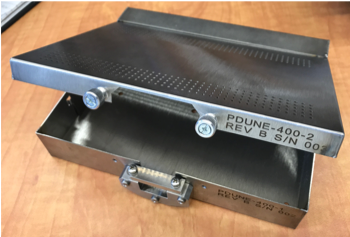
\includegraphics[width=0.45\linewidth]{tpcelec-box.png}
\end{dunefigure}
